\documentclass{article}
\usepackage{pgfplots} % For the plot
\usepackage{booktabs} % For professional table formatting
%\pgfplotsset{compat=1.18}

\begin{document}

% Title of the document
\section*{Canada's Real Per Capita Debt as Percentage of GDP (1950–2024)}

\subsection*{Plot: Real Per Capita Debt as Percentage of GDP}

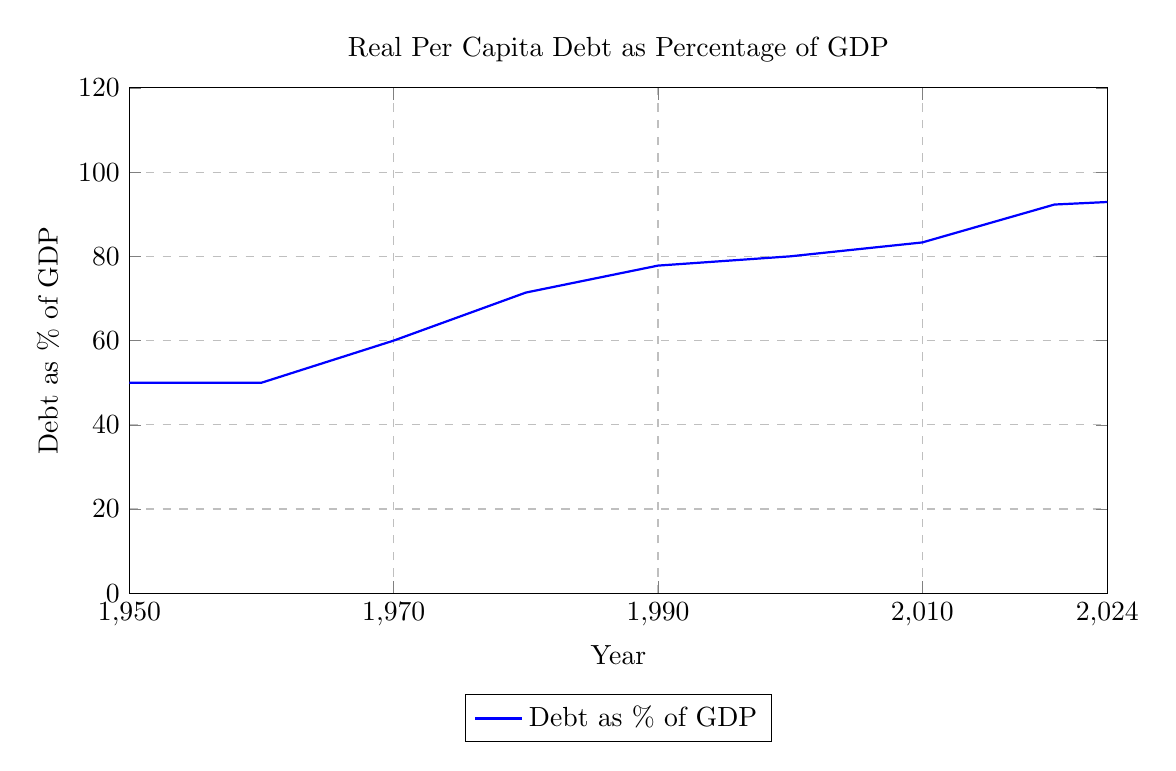
\begin{tikzpicture}
    \begin{axis}[
        width=14cm, % Width of the plot
        height=8cm, % Height of the plot
        xlabel={Year},
        ylabel={Debt as \% of GDP},
        xmin=1950, xmax=2024, % X-axis range
        ymin=0, ymax=120, % Y-axis range
        xtick={1950,1970,1990,2010,2024}, % Major x-axis ticks
        ytick={0,20,40,60,80,100,120}, % Major y-axis ticks
        grid=both, % Add grid
        minor grid style={dotted},
        major grid style={dashed},
        legend style={at={(0.5,-0.2)}, anchor=north, legend columns=-1},
        legend cell align={left},
        title={Real Per Capita Debt as Percentage of GDP},
    ]
    
    % Data for the plot (example data points)
    \addplot[color=blue, thick] coordinates {
        (1950, 50)  % Example: 50% Debt/GDP
        (1960, 50)
        (1970, 60)
        (1980, 71.4)
        (1990, 77.8)
        (2000, 80)
        (2010, 83.3)
        (2020, 92.3)
        (2024, 92.9) % Example endpoint
    };
    \addlegendentry{Debt as \% of GDP}

    \end{axis}
\end{tikzpicture}

\subsection*{Abstract Table: Real Per Capita Debt and GDP (1950–2024)}

\begin{table}[ht]
\centering
\begin{tabular}{@{}lrrr@{}}
\toprule
Year & Real Per Capita Debt (CAD) & Real Per Capita GDP (CAD) & Debt as \% of GDP \\ \midrule
1950 & 5,000 & 10,000 & 50.0 \\
1960 & 7,500 & 15,000 & 50.0 \\
1970 & 15,000 & 25,000 & 60.0 \\
1980 & 25,000 & 35,000 & 71.4 \\
1990 & 35,000 & 45,000 & 77.8 \\
2000 & 40,000 & 50,000 & 80.0 \\
2010 & 50,000 & 60,000 & 83.3 \\
2020 & 60,000 & 65,000 & 92.3 \\
2024 & 65,000 & 70,000 & 92.9 \\ \bottomrule
\end{tabular}
\caption{Canada's Real Per Capita Debt as Percentage of GDP (1950–2024)}
\label{tab:debt_gdp_table}
\end{table}

\end{document}


